\RequirePackage{fixltx2e}
\documentclass[runningheads,a4paper]{llncs}

\usepackage[american]{babel}

\usepackage{graphicx}

%extended enumerate, such as \begin{compactenum}
\usepackage{paralist}

%put figures inside a text
%\usepackage{picins}
%use
%\piccaptioninside
%\piccaption{...}
%\parpic[r]{\includegraphics ...}
%Text...

%Sorts the citations in the brackets
%\usepackage{cite}

%for easy quotations: \enquote{text}
\usepackage{csquotes}

\usepackage[T1]{fontenc}

%better font, similar to the default springer font
\usepackage{lmodern}
%if more space is needed, exchange lmodern by mathptmx
%\usepackage{mathptmx}

%enable margin kerning
\usepackage{microtype}

%for demonstration purposes only
\usepackage[math]{blindtext}

\usepackage{ifxetex,ifluatex}
\ifxetex
  \usepackage{fontspec,xltxtra,xunicode}
  \defaultfontfeatures{Mapping=tex-text,Scale=MatchLowercase}
  \newcommand{\euro}{€}
\else
  \ifluatex
    \usepackage{fontspec}
    \defaultfontfeatures{Mapping=tex-text,Scale=MatchLowercase}
    \newcommand{\euro}{€}
  \else
    \usepackage[utf8]{inputenc}
    \usepackage{eurosym}
  \fi
\fi


\makeatletter
\renewcommand\subsubsection{\@startsection{subsubsection}{3}{\z@}%
                       {-18\p@ \@plus -4\p@ \@minus -4\p@}%
                       {4\p@ \@plus 2\p@ \@minus 2\p@}%
                       {\normalfont\normalsize\bfseries\boldmath
                        \rightskip=\z@ \@plus 8em\pretolerance=10000 }}
\renewcommand\paragraph{\@startsection{paragraph}{4}{\z@}%
                       {-12\p@ \@plus -4\p@ \@minus -4\p@}%
                       {2\p@ \@plus 1\p@ \@minus 1\p@}%
                       {\normalfont\normalsize\itshape
                        \rightskip=\z@ \@plus 8em\pretolerance=10000 }}
\makeatother


%\usepackage[capitalise,nameinlink]{cleveref}
%Nice formats for \cref
%\crefname{section}{Sect.}{Sect.}
%\Crefname{section}{Section}{Sections}
%\crefname{figure}{Fig.}{Fig.}
%\Crefname{figure}{Figure}{Figures}

\usepackage{xspace}
%\newcommand{\eg}{e.\,g.\xspace}
%\newcommand{\ie}{i.\,e.\xspace}
\newcommand{\eg}{e.\,g.,\ }
\newcommand{\ie}{i.\,e.,\ }

% correct bad hyphenation here
\hyphenation{op-tical net-works semi-conduc-tor}

%%%%%%%%%%%%%%%%%%%%%%%%%%%%%%%%%%%%%%%%%%%%%%%%
\usepackage{fancyvrb}
%\DefineShortVerb[commandchars=\\\{\}]{\|}
\DefineVerbatimEnvironment{Highlighting}{Verbatim}{commandchars=\\\{\}}
% Add ',fontsize=\small' for more characters per line
\newenvironment{Shaded}{}{}
\newcommand{\KeywordTok}[1]{\textcolor[rgb]{0.00,0.44,0.13}{\textbf{{#1}}}}
\newcommand{\DataTypeTok}[1]{\textcolor[rgb]{0.56,0.13,0.00}{{#1}}}
\newcommand{\DecValTok}[1]{\textcolor[rgb]{0.25,0.63,0.44}{{#1}}}
\newcommand{\BaseNTok}[1]{\textcolor[rgb]{0.25,0.63,0.44}{{#1}}}
\newcommand{\FloatTok}[1]{\textcolor[rgb]{0.25,0.63,0.44}{{#1}}}
\newcommand{\CharTok}[1]{\textcolor[rgb]{0.25,0.44,0.63}{{#1}}}
\newcommand{\StringTok}[1]{\textcolor[rgb]{0.25,0.44,0.63}{{#1}}}
\newcommand{\CommentTok}[1]{\textcolor[rgb]{0.38,0.63,0.69}{\textit{{#1}}}}
\newcommand{\OtherTok}[1]{\textcolor[rgb]{0.00,0.44,0.13}{{#1}}}
\newcommand{\AlertTok}[1]{\textcolor[rgb]{1.00,0.00,0.00}{\textbf{{#1}}}}
\newcommand{\FunctionTok}[1]{\textcolor[rgb]{0.02,0.16,0.49}{{#1}}}
\newcommand{\RegionMarkerTok}[1]{{#1}}
\newcommand{\ErrorTok}[1]{\textcolor[rgb]{1.00,0.00,0.00}{\textbf{{#1}}}}
\newcommand{\NormalTok}[1]{{#1}}
\ifxetex
  \usepackage[setpagesize=false, % page size defined by xetex
              unicode=false, % unicode breaks when used with xetex
              xetex,
              colorlinks=true,
              linkcolor=blue]{hyperref}
\else
%  \usepackage[unicode=true,
%              colorlinks=true,
%              linkcolor=blue]{hyperref}
    %unobstrusive usage of hyperref
    \ifnum\pdfoutput>0
        \usepackage[
        unicode=true,
        %pdfauthor={},
        %pdfsubject={},
        %pdftitle={},
        %pdfkeywords={},
        bookmarks=false,
        breaklinks=true,
        colorlinks=true,
        linkcolor=black,
        citecolor=black,
        urlcolor=black,
        %pdfstartpage=19,
        pdfpagelayout=SinglePage
        ]{hyperref}
        %enables correct jumping to figures when referencing
        \usepackage[all]{hypcap}
    \else
        \usepackage{hyperref}
    \fi
\fi
\hypersetup{breaklinks=true, pdfborder={0 0 0}}
\setlength{\parindent}{15pt} % set to 0pt if you want no indent in the first line of a paragraph
%\setlength{\parskip}{6pt plus 2pt minus 1pt}
\setlength{\parskip}{0pt}
\setlength{\emergencystretch}{3em}  % prevent overfull lines
\setcounter{secnumdepth}{3}
%\EndDefineVerbatimEnvironment{Highlighting}

\raggedbottom % allow ragged page bottoms

\def\tightlist{} % fix error when translating md lists to itemize

%%%%%%%%%%%%%%%%%%%%%%%%%%%%%%%%%%%%%%%%%%%%%%%%

\begin{document}

%Works on MiKTeX only
%hint by http://goemonx.blogspot.de/2012/01/pdflatex-ligaturen-und-copynpaste.html
%This allows a copy'n'paste of the text from the paper
\input glyphtounicode.tex
\pdfgentounicode=1

\title{My title}
%If Title is too long, use \titlerunning
%\titlerunning{Short Title}
%Single insitute
\author{Firstname Lastname}

%If there are too many authors, use \authorrunning
%\authorrunning{First Author et al.}


\institute{
\email{\href{mailto:optional@email.com}{\nolinkurl{optional@email.com}}}
\\My optional Institute
\\My optional University
}

%Multiple insitutes
%Currently disabled
%
\iffalse
\authorinfo{
  
}{
}{
  \{\}
}
\fi


\maketitle

	\begin{abstract}
		Lorem ipsum dolor sit amet, consetetur sadipscing elitr, sed diam nonumy
eirmod tempor invidunt ut labore et dolore magna aliquyam erat, sed diam
voluptua.
	\end{abstract}

	\keywords{Lorem, Ipsum}

\section{Story Line}\label{story-line}

\begin{itemize}
\tightlist
\item
  Test Time Generation - Directed Random is faster in regards to AVM and
  AVM-Defaults.
\item
  Coverage - As Directed Random is faster it has the same coverage as
  the rest of the techniques.
\item
  Mutation Score - Directed Random has the higher or similar mutation
  score comparing to AVM and AVM-Defaults.
\end{itemize}

\section{RQs}\label{rqs}

\subsection{Test Time Generation}\label{test-time-generation}

How efficent Directed Random in regard of test time generation comparing
to the other data generators?

\subsection{Coverage}\label{coverage}

How do the number of test requirements generated by the coverage
criteria differ depending on the data generation technique being used,
and how successfully can test cases be automatically generated to
satisfy them?

\subsection{Fault-Finding
Effectiveness}\label{fault-finding-effectiveness}

How does fault finding effectiveness vary depending on data generation
technique used?

\section{What Plots ?}\label{what-plots}

\subsection{Test time generation
(Effiency)}\label{test-time-generation-effiency}

\subsubsection{Analyse Wilcox Rank and Effect Size for AVM and Directed
Random}\label{analyse-wilcox-rank-and-effect-size-for-avm-and-directed-random}

To statistically analyze the the new technique we conducted tests for
significance with the nonparametric Wilcoxon rank-sum test, using the
sets of 30 execution times obtained with a specific DBMS and all
techniques \textbf{Hitchhicker Guide Ref}. A p-value that less than
\(0.05\) is considered significant. To review practical are significance
tests we use the nonparametric A12 statistic of Vargha and Delaney
\textbf{REF} was used to calculate effect sizes. The A12 determine the
average probability that one approach beats another, or how superior one
technique compared to the other. We followed the guidelines of Vargha
and Delaney in that an effect size is considered to be \enquote{large}
if the value of A12 is \$ \textless{} 0:29\$ or \(> 0.71\),
\enquote{medium} if A12 is \(< 0.36\) or \(> 0.64\) and \enquote{small}
if A12 is \(< 0.44\) or \(> 0.56\). However, is the values of A12 close
to the 0.5 value are viewed as there no effect.

When comparing AVM and Directed Random techniques in regard of time we
used Mann-Whitney U-test and the A-hat effect size calculations. As
Shown in in the following two tables that there is statistically
significat differance between Driected Random and AVM, \(p \leq 0.05\).
Therefore, we reject the null hypothesis that there is no difference
between AVM and Directed Random. As p-value near zero, that directed
random is faster than AVM in a statistically significant test. Moreover,
the A-12 shows that Directed Random has a large effect size when it
comes to test generation timing. Which menas that Directed Random is the
winner in regard of test generation timing.

\begin{tabular}{r|l}
\hline
p.value & dbms\\
\hline
0 & Postgres\\
\hline
0 & SQLite\\
\hline
0 & HyperSQL\\
\hline
\end{tabular}

Figure 1 and 2.

\begin{figure}[h]
\centering
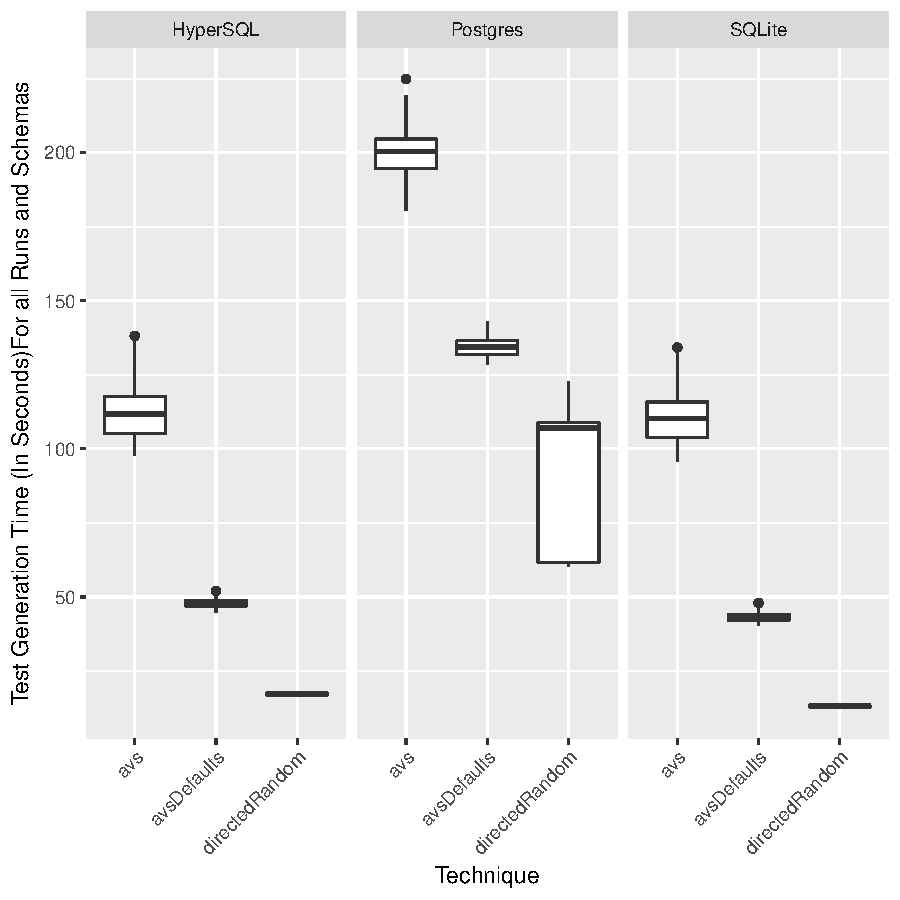
\includegraphics[width=\linewidth]{../plots/figure3.pdf}
\caption{Test generation timing - in seconds. First summing test
generation timing for each run then group by data generator and DBMS,
then divide test generation timing by 1000 to convert to second.}
\end{figure}

\begin{figure}[h]
	\centering
	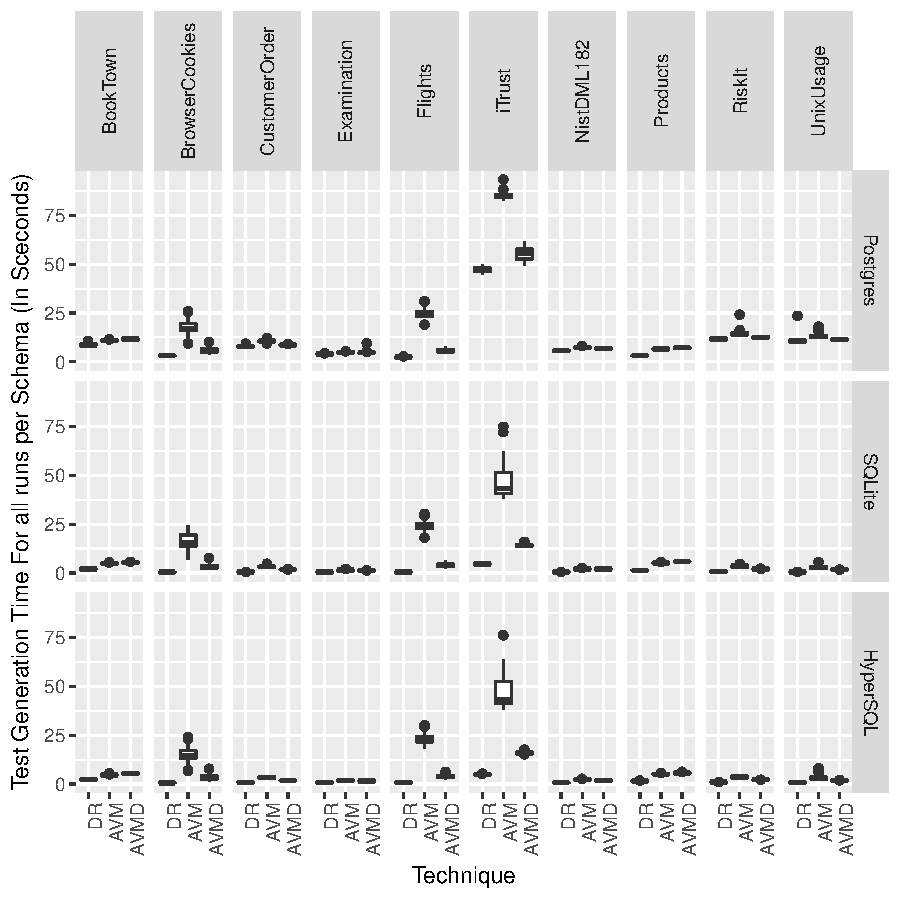
\includegraphics[width=\linewidth]{../plots/figure24.pdf}
	\caption{Test generation timing box plot showing some of Game Changer schemas}
\end{figure}

\begin{figure}[h]
\centering
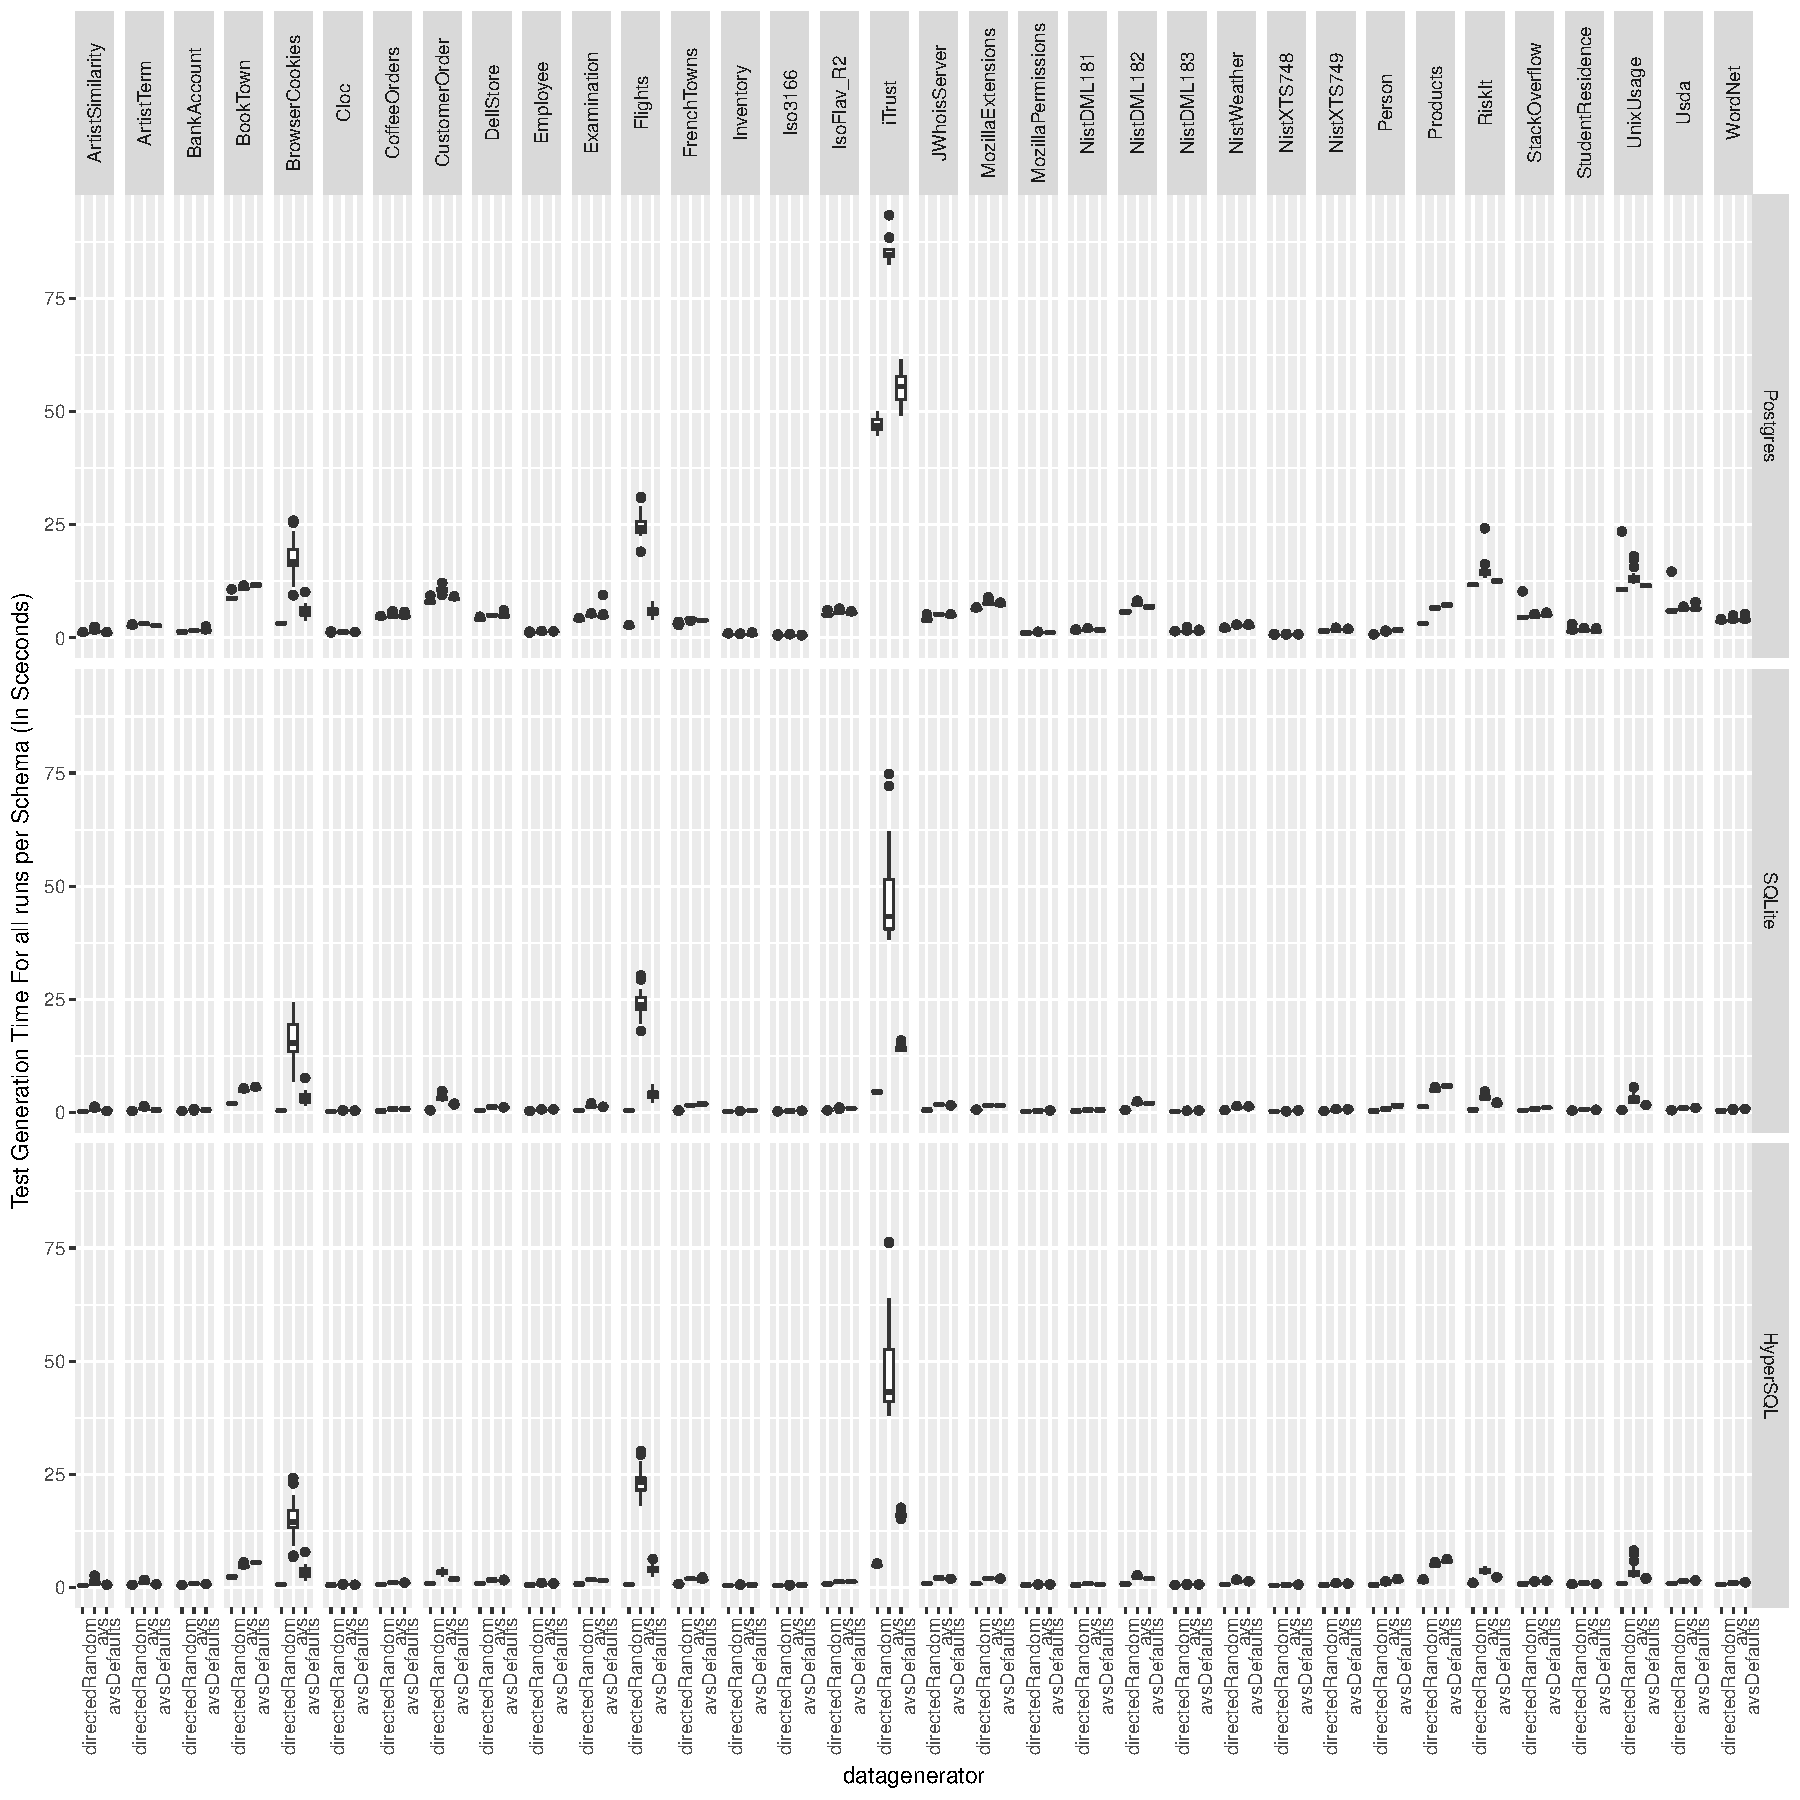
\includegraphics[width=\linewidth]{../plots/figure4.pdf}
\caption{Box plot for Test Generation time for DBMS, techniques and
schemas - in precentage. Group by data generator, case study and DBMS,
then dividing test generation timning by 1000 to convert to second. No
averaging or summing to see the spread of values for all runs per
schema}
\end{figure}

\subsection{Coverage}\label{coverage-1}

Figure 3 and 4.

\begin{figure}[h]
	\centering
	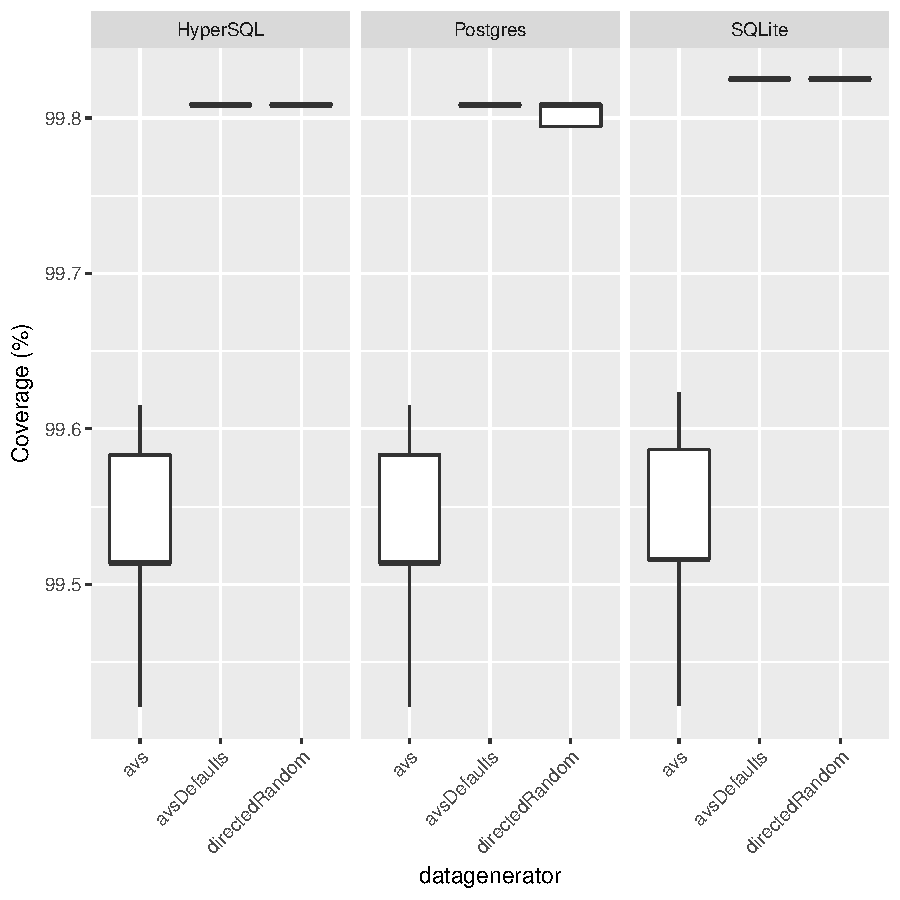
\includegraphics[width=\linewidth]{../plots/figure23.pdf}
	\caption{Box plot for Coverage, averaging all schema coverage per run}
\end{figure}

\begin{figure}[h]
\centering
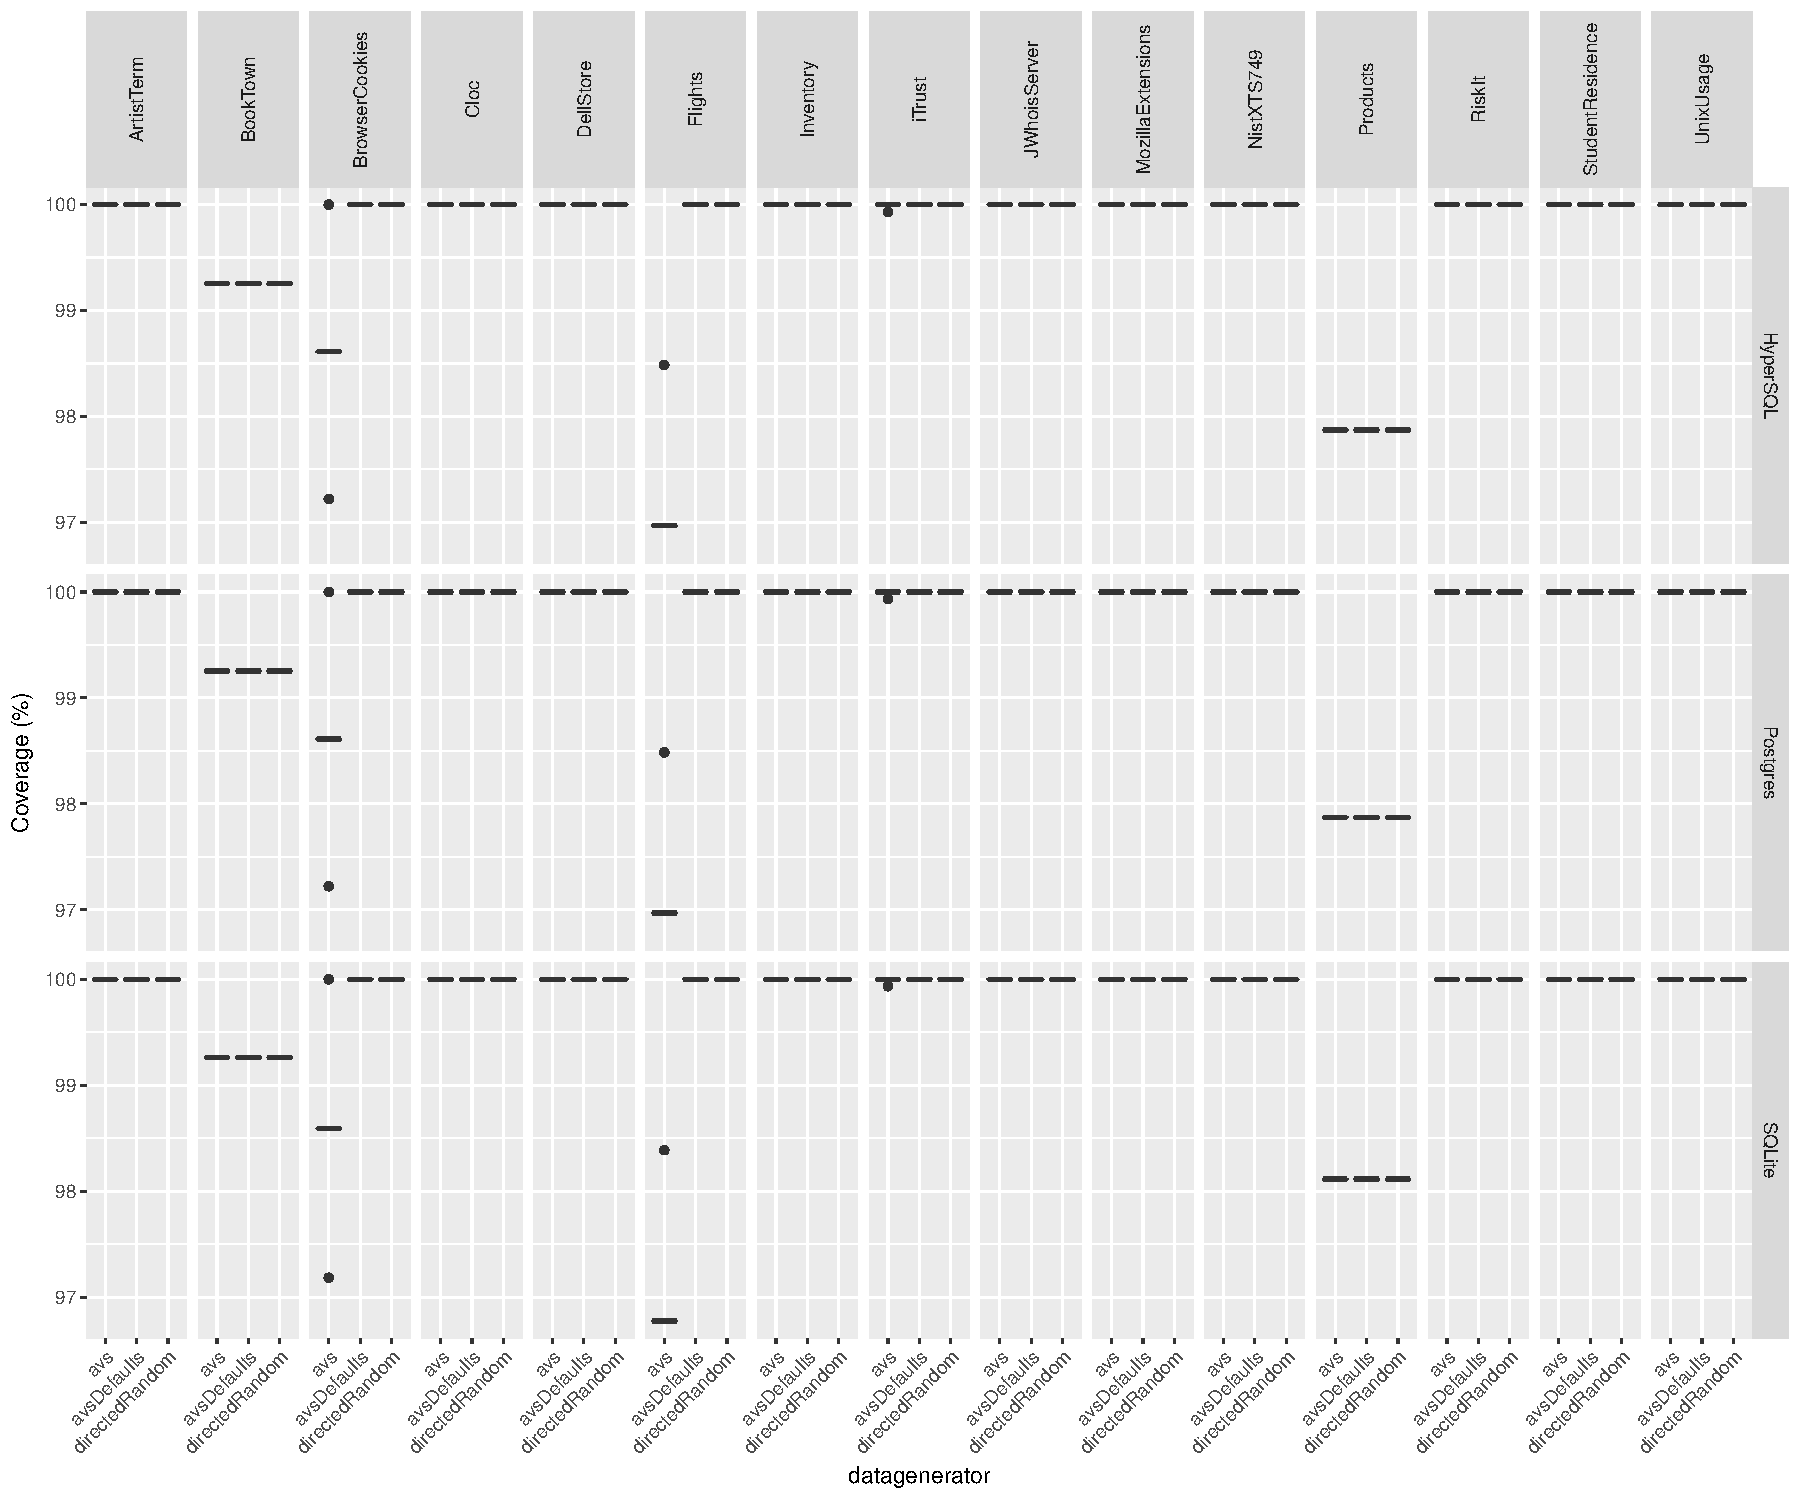
\includegraphics[width=\linewidth]{../plots/figure22.pdf}
\caption{Box plot for Coverage}
\end{figure}

\subsection{Mutation Score}\label{mutation-score}

Figure 5, 6 and 7.

\begin{itemize}
	\item Directed Random has a higher PKColumnA operator kills than AVM-Defaults.
	\item Primary Key Composite key can be problematic for AV<-Defaults.
	\item Directed Random has either similar or less (because of coverage) mutation kill compared to AVM.
	\item AVM has lower coverage than AVM-Defaults however it has a higher mutation score because of empty strings and Composite keys.
\end{itemize}

\begin{figure}[h]
\centering
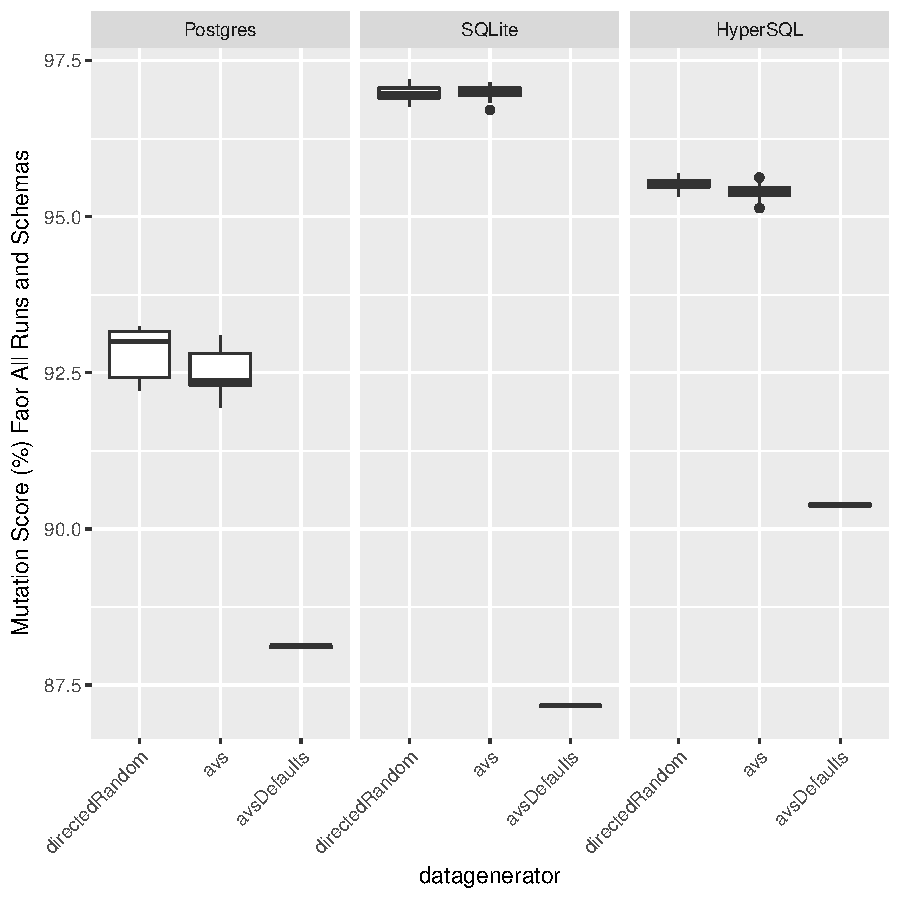
\includegraphics[width=\linewidth]{../plots/figure7.pdf}
\caption{Box plot for mutation scores for DBMSs and techniques - in
precentage. Frist I sum all score numerator and denominator per run per
DBMS per data generator, then plottig using group by data generator,
DBMS and divding the score numerator by denominator multiplying by 100}
\end{figure}

\begin{figure}[h]
\centering
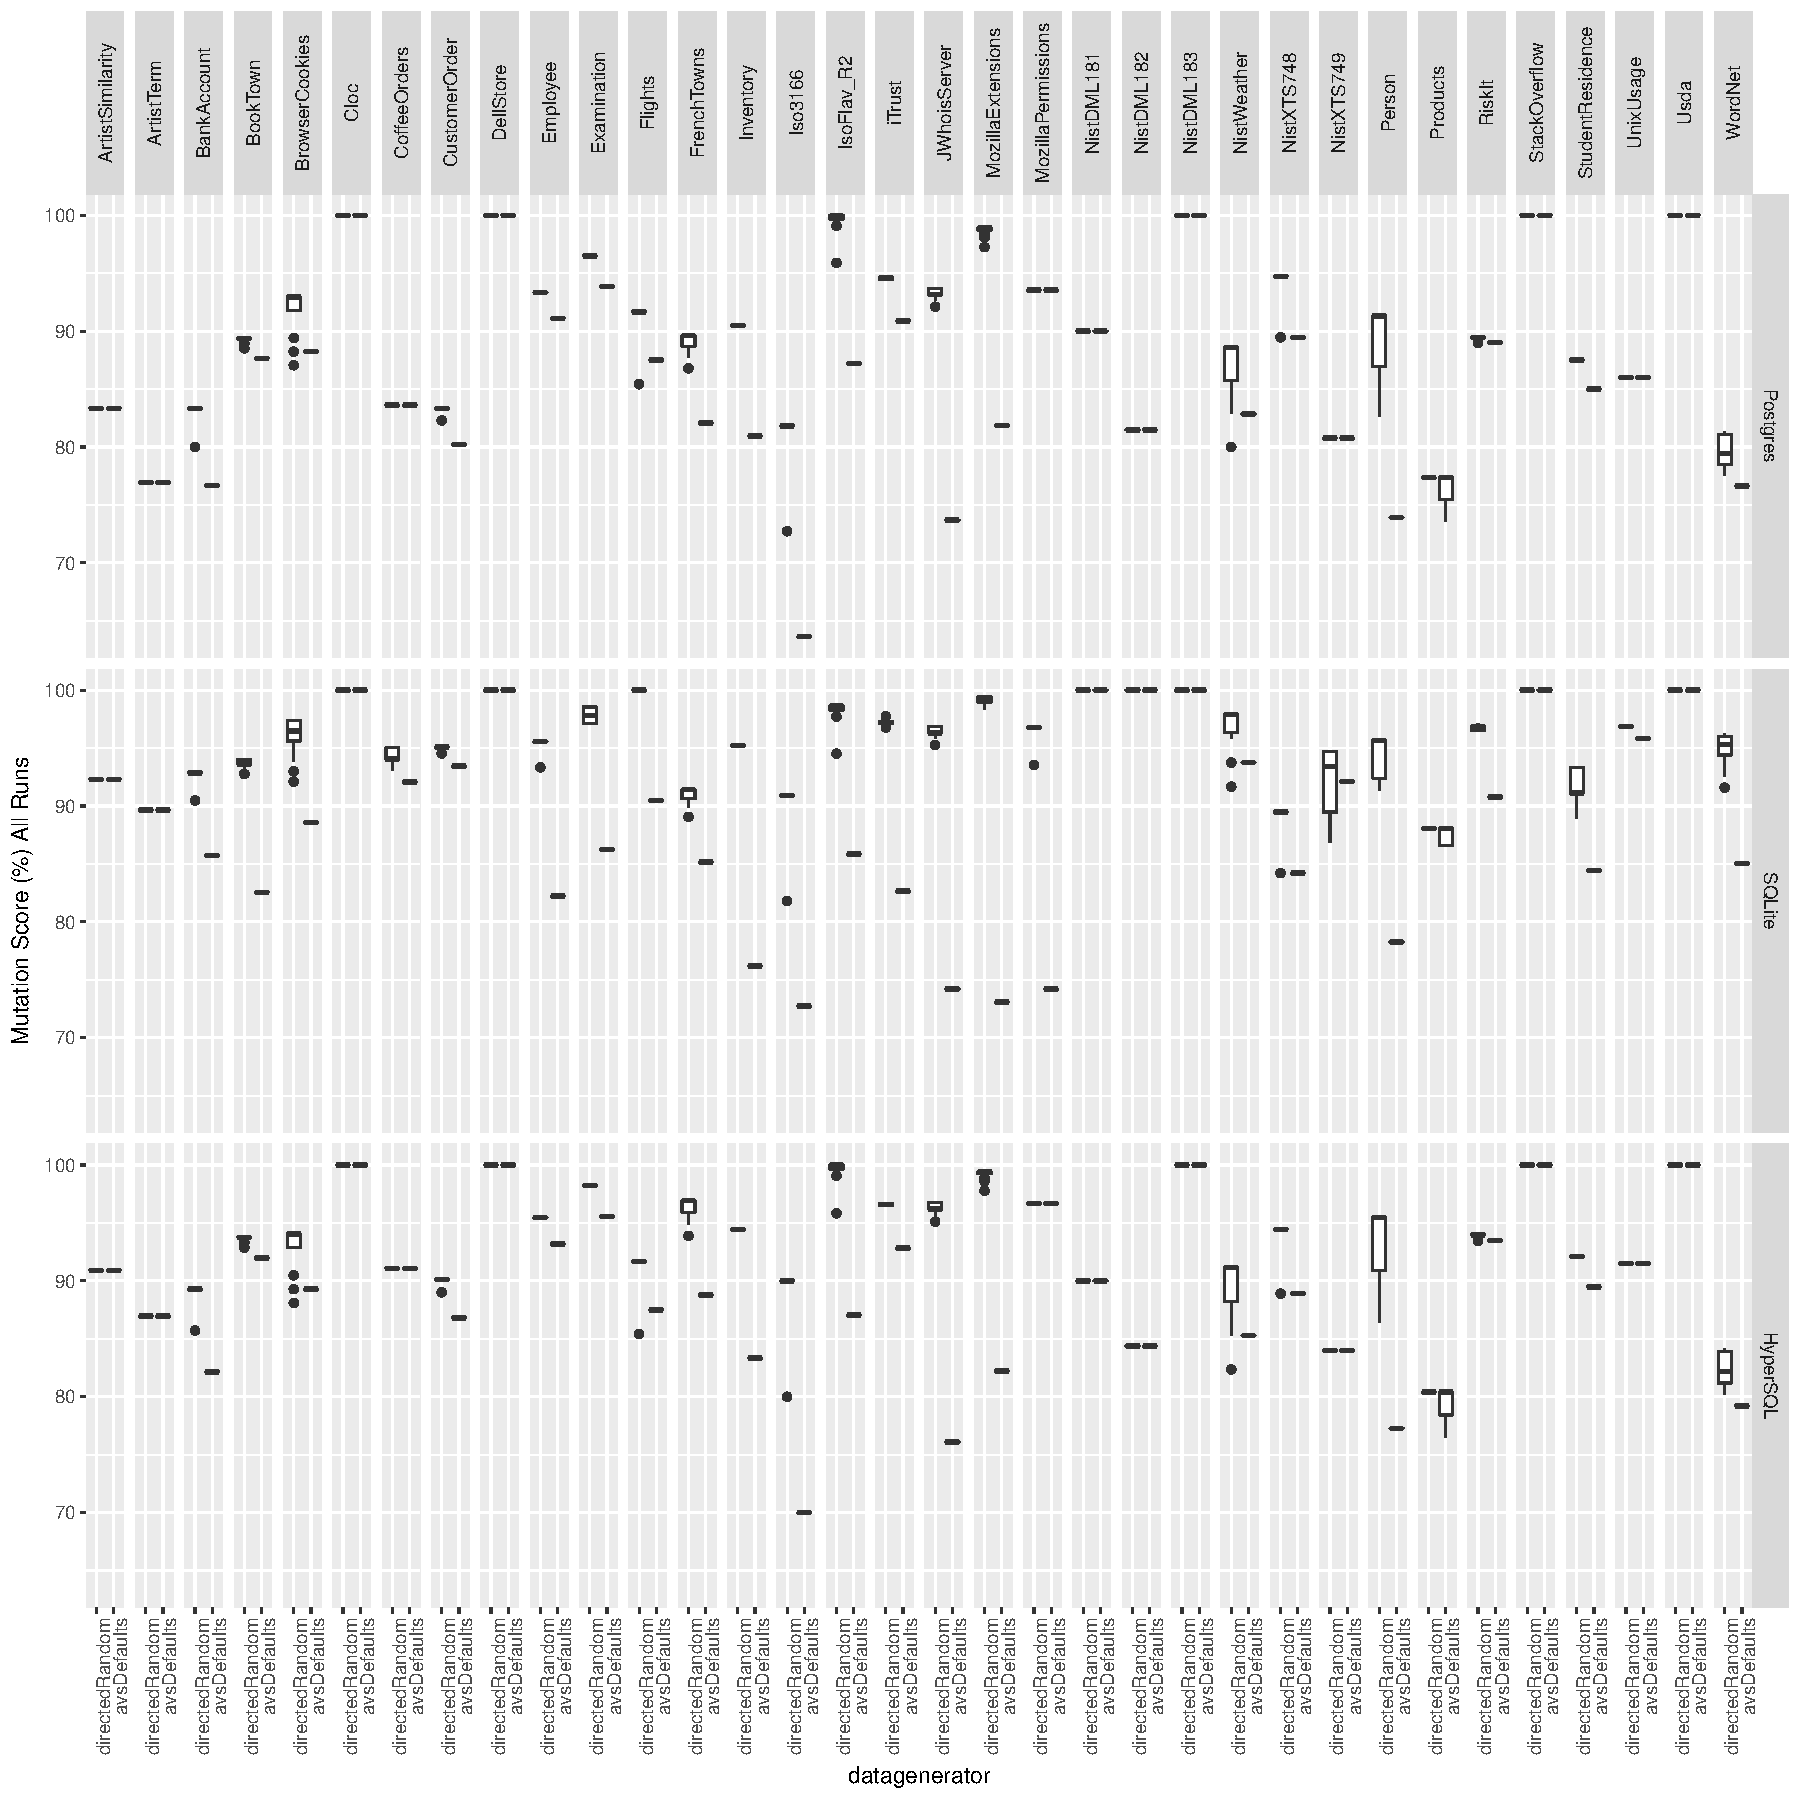
\includegraphics[width=\linewidth]{../plots/figure8.pdf}
\caption{Box plot for mutation scores for DBMS, techniques and schemas -
in precentage. Group by data generator, case study and DBMS, then
divding the score numerator by denominator multiplying by 100. No
averaging or summing to see the spread of values for all runs per
schema}
\end{figure}

\begin{figure}[h]
\centering
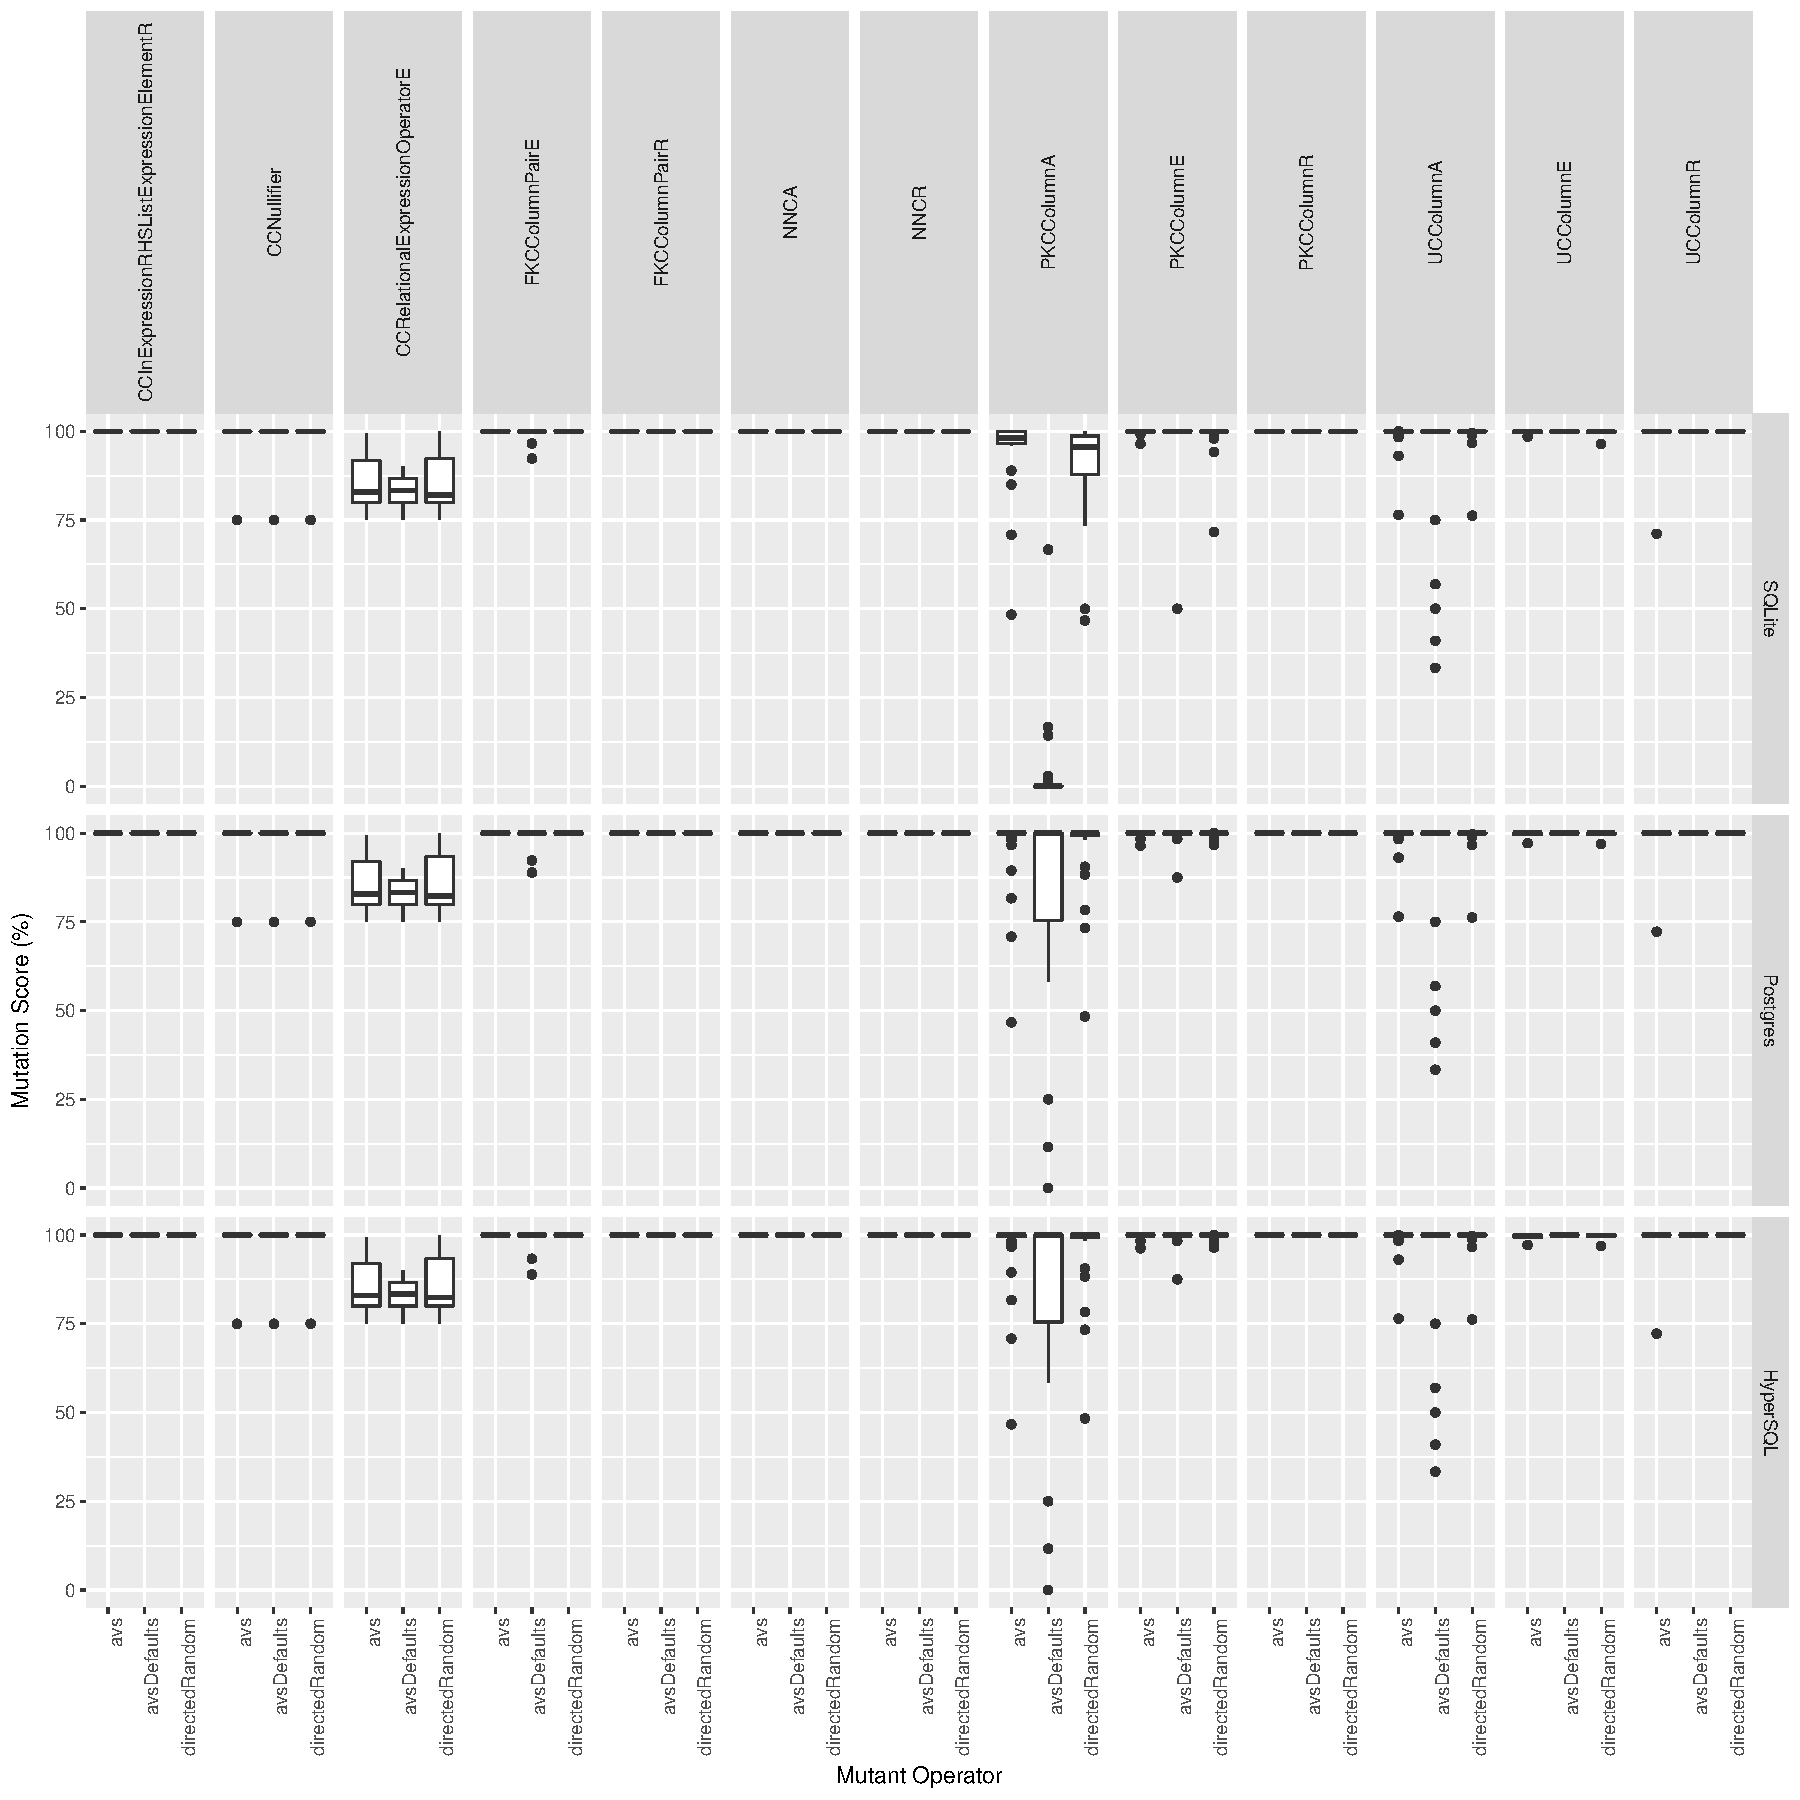
\includegraphics[width=\linewidth]{../plots/figure10.pdf}
\caption{Box Plot of mutant scores in regard of Mutant Operators and
DBMSs - in precentage. Using mutanttiming file, I group by generator,
DBMS, schema and operator. Then I only select NORMAL mutants, then
calculating the percentage of killed mutant by summing all killed
divided by (killed mutant plus alive mutant) multiply by 100.}
\end{figure}

\newpage
\begin{table}
	\begin{center}
	\scalebox{0.9}{
	\begin{tabular}{lccc|ccc|ccc}
		\hline
		& \multicolumn{3}{c}{Postgres} & \multicolumn{3}{c}{SQLite} & \multicolumn{3}{c}{HyperSQL} \\ 
		Case Study  & DR & AVM & AVMD & DR & AVM & AVMD & DR & AVM &  \multicolumn{1}{c}{AVMD} \\ 
		\hline
		ArtistSimilarity  & $\phantom{0}1019.9$ & $\phantom{0}1406.4$ & $\phantom{0}1079.7$ & $\phantom{0}288.6$ & $\phantom{00}717.5$ & $\phantom{00}444.7$ & $\phantom{0}492.4$ & $\phantom{00}961.7$ & $\phantom{00}598.4$ \\
		ArtistTerm  & $\phantom{0}2603.4$ & $\phantom{0}3103.9$ & $\phantom{0}2679.6$ & $\phantom{0}327.6$ & $\phantom{00}913.9$ & $\phantom{00}541.5$ & $\phantom{0}555.3$ & $\phantom{0}1152.7$ & $\phantom{00}718.8$ \\
		BankAccount  & $\phantom{0}1327.0$ & $\phantom{0}1619.6$ & $\phantom{0}1588.5$ & $\phantom{0}321.9$ & $\phantom{00}624.8$ & $\phantom{00}574.6$ & $\phantom{0}533.7$ & $\phantom{00}834.9$ & $\phantom{00}756.1$ \\
		BookTown  & $\phantom{0}8780.0$ & $10940.0$ & $11587.8$ & $2002.3$ & $\phantom{0}4908.5$ & $\phantom{0}5443.3$ & $2345.7$ & $\phantom{0}4634.5$ & $\phantom{0}5491.0$ \\
		BrowserCookies  & $\phantom{0}3215.2$ & $17499.5$ & $\phantom{0}5849.8$ & $\phantom{0}419.3$ & $15703.0$ & $\phantom{0}3234.6$ & $\phantom{0}657.6$ & $15044.5$ & $\phantom{0}3366.1$ \\
		Cloc  & $\phantom{0}1149.2$ & $\phantom{0}1275.7$ & $\phantom{0}1192.6$ & $\phantom{0}302.7$ & $\phantom{00}408.6$ & $\phantom{00}433.2$ & $\phantom{0}514.4$ & $\phantom{00}631.4$ & $\phantom{00}599.4$ \\
		CoffeeOrders  & $\phantom{0}4429.6$ & $\phantom{0}4898.4$ & $\phantom{0}4743.9$ & $\phantom{0}398.2$ & $\phantom{00}849.1$ & $\phantom{00}823.6$ & $\phantom{0}653.6$ & $\phantom{0}1105.7$ & $\phantom{0}1078.6$ \\
		CustomerOrder  & $\phantom{0}7944.4$ & $10622.1$ & $\phantom{0}8647.8$ & $\phantom{0}545.4$ & $\phantom{0}3217.7$ & $\phantom{0}1789.3$ & $\phantom{0}863.6$ & $\phantom{0}3364.1$ & $\phantom{0}1870.2$ \\
		DellStore  & $\phantom{0}4186.7$ & $\phantom{0}4955.1$ & $\phantom{0}4844.9$ & $\phantom{0}483.9$ & $\phantom{0}1276.7$ & $\phantom{0}1137.1$ & $\phantom{0}829.6$ & $\phantom{0}1632.1$ & $\phantom{0}1562.4$ \\
		Employee  & $\phantom{0}1045.3$ & $\phantom{0}1271.7$ & $\phantom{0}1340.6$ & $\phantom{0}341.1$ & $\phantom{00}592.5$ & $\phantom{00}700.6$ & $\phantom{0}552.8$ & $\phantom{00}815.8$ & $\phantom{00}898.7$ \\
		Examination  & $\phantom{0}4052.1$ & $\phantom{0}4938.5$ & $\phantom{0}4835.7$ & $\phantom{0}488.3$ & $\phantom{0}1448.5$ & $\phantom{0}1267.8$ & $\phantom{0}784.3$ & $\phantom{0}1737.6$ & $\phantom{0}1569.1$ \\
		Flights  & $\phantom{0}2483.6$ & $24840.6$ & $\phantom{0}5771.7$ & $\phantom{0}453.6$ & $24019.3$ & $\phantom{0}3904.0$ & $\phantom{0}690.0$ & $23295.5$ & $\phantom{0}3989.1$ \\
		FrenchTowns  & $\phantom{0}3022.7$ & $\phantom{0}4171.4$ & $\phantom{0}3860.3$ & $\phantom{0}429.4$ & $\phantom{0}1628.6$ & $\phantom{0}1938.0$ & $\phantom{0}683.0$ & $\phantom{0}1941.1$ & $\phantom{0}1699.5$ \\
		Inventory  & $\phantom{00}696.7$ & $\phantom{00}751.5$ & $\phantom{00}801.8$ & $\phantom{0}283.7$ & $\phantom{00}353.9$ & $\phantom{00}436.5$ & $\phantom{0}481.6$ & $\phantom{00}555.6$ & $\phantom{00}601.7$ \\
		Iso3166  & $\phantom{00}476.8$ & $\phantom{00}544.4$ & $\phantom{00}500.5$ & $\phantom{0}274.9$ & $\phantom{00}353.0$ & $\phantom{00}402.7$ & $\phantom{0}472.4$ & $\phantom{00}547.7$ & $\phantom{00}546.4$ \\
		IsoFlav\_R2  & $\phantom{0}5125.8$ & $\phantom{0}5685.0$ & $\phantom{0}5479.2$ & $\phantom{0}432.4$ & $\phantom{00}986.1$ & $\phantom{00}932.7$ & $\phantom{0}754.8$ & $\phantom{0}1311.2$ & $\phantom{0}1265.6$ \\
		iTrust  & $46962.1$ & $85790.2$ & $55277.0$ & $4583.8$ & $47114.7$ & $14124.8$ & $4910.9$ & $47908.5$ & $15985.8$ \\
		JWhoisServer  & $\phantom{0}4031.4$ & $\phantom{0}5154.1$ & $\phantom{0}4874.0$ & $\phantom{0}550.3$ & $\phantom{0}1786.9$ & $\phantom{0}1550.1$ & $\phantom{0}890.2$ & $\phantom{0}2085.7$ & $\phantom{0}1876.9$ \\
		MozillaExtensions  & $\phantom{0}6358.3$ & $\phantom{0}7616.2$ & $\phantom{0}7339.4$ & $\phantom{0}545.5$ & $\phantom{0}1647.0$ & $\phantom{0}1554.6$ & $\phantom{0}863.3$ & $\phantom{0}2009.3$ & $\phantom{0}1916.8$ \\
		MozillaPermissions  & $\phantom{0}1077.1$ & $\phantom{0}1162.0$ & $\phantom{0}1190.4$ & $\phantom{0}307.9$ & $\phantom{00}404.9$ & $\phantom{00}492.0$ & $\phantom{0}513.4$ & $\phantom{00}608.7$ & $\phantom{00}663.4$ \\
		NistDML181  & $\phantom{0}1553.9$ & $\phantom{0}1800.9$ & $\phantom{0}1706.7$ & $\phantom{0}317.2$ & $\phantom{00}617.4$ & $\phantom{00}540.4$ & $\phantom{0}528.3$ & $\phantom{00}834.9$ & $\phantom{00}706.2$ \\
		NistDML182  & $\phantom{0}5737.0$ & $\phantom{0}7429.5$ & $\phantom{0}6811.2$ & $\phantom{0}501.3$ & $\phantom{0}2097.4$ & $\phantom{0}2087.6$ & $\phantom{0}761.8$ & $\phantom{0}2363.4$ & $\phantom{0}1942.0$ \\
		NistDML183  & $\phantom{0}1321.5$ & $\phantom{0}1438.0$ & $\phantom{0}1441.7$ & $\phantom{0}295.5$ & $\phantom{00}359.8$ & $\phantom{00}475.2$ & $\phantom{0}510.4$ & $\phantom{00}577.0$ & $\phantom{00}638.1$ \\
		NistWeather  & $\phantom{0}1934.3$ & $\phantom{0}2642.7$ & $\phantom{0}2517.5$ & $\phantom{0}481.2$ & $\phantom{0}1138.2$ & $\phantom{0}1216.9$ & $\phantom{0}709.9$ & $\phantom{0}1421.5$ & $\phantom{0}1312.6$ \\
		NistXTS748  & $\phantom{00}613.9$ & $\phantom{00}659.2$ & $\phantom{00}706.9$ & $\phantom{0}278.0$ & $\phantom{00}331.3$ & $\phantom{00}501.4$ & $\phantom{0}475.4$ & $\phantom{00}534.1$ & $\phantom{00}613.9$ \\
		NistXTS749  & $\phantom{0}1535.2$ & $\phantom{0}1807.8$ & $\phantom{0}1772.5$ & $\phantom{0}326.8$ & $\phantom{00}566.2$ & $\phantom{00}693.5$ & $\phantom{0}546.0$ & $\phantom{00}775.9$ & $\phantom{00}823.5$ \\
		Person  & $\phantom{00}677.8$ & $\phantom{0}1170.4$ & $\phantom{0}1728.4$ & $\phantom{0}341.8$ & $\phantom{00}866.4$ & $\phantom{0}1563.3$ & $\phantom{0}546.1$ & $\phantom{0}1050.8$ & $\phantom{0}1599.0$ \\
		Products  & $\phantom{0}3135.5$ & $\phantom{0}6610.6$ & $\phantom{0}7279.2$ & $1310.6$ & $\phantom{0}5029.1$ & $\phantom{0}5852.2$ & $1519.4$ & $\phantom{0}5004.2$ & $\phantom{0}5796.4$ \\
		RiskIt  & $11696.2$ & $14718.1$ & $12527.7$ & $\phantom{0}630.5$ & $\phantom{0}3475.7$ & $\phantom{0}1987.6$ & $\phantom{0}996.6$ & $\phantom{0}3619.7$ & $\phantom{0}2312.9$ \\
		StackOverflow  & $\phantom{0}4662.2$ & $\phantom{0}4828.1$ & $\phantom{0}5010.0$ & $\phantom{0}480.6$ & $\phantom{00}841.9$ & $\phantom{0}1124.2$ & $\phantom{0}816.4$ & $\phantom{0}1169.1$ & $\phantom{0}1474.7$ \\
		StudentResidence  & $\phantom{0}1429.8$ & $\phantom{0}1720.3$ & $\phantom{0}1539.8$ & $\phantom{0}383.6$ & $\phantom{00}750.6$ & $\phantom{00}628.4$ & $\phantom{0}592.8$ & $\phantom{00}965.5$ & $\phantom{00}782.6$ \\
		UnixUsage  & $11108.9$ & $13308.4$ & $11523.3$ & $\phantom{0}524.2$ & $\phantom{0}2988.5$ & $\phantom{0}1674.1$ & $\phantom{0}866.6$ & $\phantom{0}3479.7$ & $\phantom{0}1925.2$ \\
		Usda  & $\phantom{0}6231.0$ & $\phantom{0}6397.2$ & $\phantom{0}6474.4$ & $\phantom{0}491.0$ & $\phantom{0}1007.2$ & $\phantom{0}1027.8$ & $\phantom{0}864.7$ & $\phantom{0}1400.6$ & $\phantom{0}1526.3$ \\
		WordNet  & $\phantom{0}3635.8$ & $\phantom{0}3918.2$ & $\phantom{0}3985.0$ & $\phantom{0}398.8$ & $\phantom{00}665.0$ & $\phantom{00}836.0$ & $\phantom{0}679.2$ & $\phantom{00}967.9$ & $\phantom{0}1125.1$ \\
		\hline 
	\end{tabular}}
\end{center}
\caption{Table}
\end{table}
\hypertarget{refs}{}

\end{document}
